%%%%%%%%%%%%%%%%%%%%%%%%%%%%%%%%%%%%%%%%%%%%%%%%%%%%%%%%%%%%%%%%%%%%%%
% Lớp 10 | Bất phương trình bậc 2 một ẩn | Dấu của tam thức bậc 2
% Dạng 0D7?1-5: Toán thực tế  ứng dụng dấu tam thức bậc 2
% Số câu: 3  (sinh tự động bởi tach_cau.py; từ nay thầy sửa trực tiếp file này)
%%%%%%%%%%%%%%%%%%%%%%%%%%%%%%%%%%%%%%%%%%%%%%%%%%%%%%%%%%%%%%%%%%%%%%

%%%%%%%%%%%%%%%% ĐÚNG/SAI %%%%%%%%%%%%%%%%

% nguồn: MaHoaNH_DungSai_Lop10
\begin{ex}%[0D7H1-5]%[ma:9f03b68a]
	Để xây dựng phương án kinh doanh cho một loại sản phẩm, doanh nghiệp tính toán lợi  nhuận $y$ (đồng) theo công thức sau: $y = -86x^2 + 86\,000x - 18\,146\,000$, trong đó $x$ là số sản phẩm được bán ra.
	\choiceTF 
		{Doanh nghiệp bị lỗ khi bán từ  $303$ đến $698$ sản phẩm}
		{Doanh nghiệp có lãi khi bán tối  đa $302$ sản phẩm hoặc bán tối thiểu $697$ sản phẩm}
		{\True Doanh nghiệp có  lãi khi bán từ $303$ đến $697$ sản phẩm}
		{\True Doanh nghiệp bị  lỗ khi bán tối đa $302$ sản phẩm hoặc bán tối thiểu $698$ sản phẩm}
	 \loigiai{Xét tam thức bậc hai $f(x) = -86x^2 + 86\,000x - 18\,146\,000$.\\
		Nhận thấy $f(x) = 0$ có hai nghiệm là  $x_1 \approx 302{,}5$; $x_2 \approx 697{,}5$ và hệ số $a = -86 < 0$.\\
		Ta có bảng  xét dấu
		\begin{center}
			\begin{tikzpicture}
					 \tkzTabInit[nocadre=true,deltacl=0.5,espcl=2.5,lgt=2]
						{$x$/1,$f (x)$/1} 
						{$-\infty$,$x_1$,$x_2$,$+\infty$} 
					\tkzTabLine{,-,0,+,0,-,} 
				\end{tikzpicture}
		\end{center}
		 Vì $x$ là số nguyên dương nên
		\begin{itemize}
			\item Doanh nghiệp có lãi khi và chỉ khi $f(x)  > 0$, tức là $303 \le x \le 697$.
			\item Doanh nghiệp bị lỗ khi và chỉ khi $f(x) < 0$, tức là $x \le 302$ hoặc $x \ge 698$. 
		\end{itemize}
		Vậy doanh  nghiệp có lãi khi bán từ $303$ đến $697$ sản phẩm, doanh nghiệp bị lỗ khi bán tối đa $302$ sản phẩm hoặc bán tối thiểu $698$ sản phẩm.
} 
\end{ex}

% nguồn: MaHoaNH_DungSai_Lop10
\begin{ex}%[0D7V1-5]%[ma:dff65b60]
	Một cửa hàng sách mua sách từ nhà xuất bản với  giá $50$ (nghìn đồng)/cuốn. Cửa hàng ước tính rằng, nếu bán $1$ cuốn sách với giá là $x$ (nghìn đồng) thì mỗi tháng khách hàng sẽ mua $(150-x)$ cuốn sách.
	\choiceTF 
		{ Theo ước tính, nếu  cửa hàng bán một cuốn sách giá $80$ nghìn đồng
		thì mỗi  tháng khách hàng sẽ mua $150$ cuốn sách}
		{\True Số tiền lãi của cửa hàng mỗi tháng được tính bằng  công thức
		$T(x)=-x^2+200x-7\,500$} 
		{Cửa hàng sẽ đạt lợi  nhuận $2{,}1$ triệu đồng mỗi tháng nếu mỗi tháng
		khách  hàng mua $80$ cuốn sách}
		{\True Nếu cửa  hàng bán một cuốn sách với giá $100$ nghìn đồng thì sẽ có lợi
		 nhuận cao nhất}
	 \loigiai{
		\begin{itemchoice}
			\itemch Theo ước tính, nếu cửa hàng bán một cuốn sách giá $80$ nghìn đồng thì mỗi tháng khách hàng  sẽ mua $150$ cuốn sách.\\
			Nếu  cửa hàng bán một cuốn sách giá $80$ nghìn đồng thì mỗi tháng khách hàng sẽ mua $150-80=70$ cuốn sách.
			\itemch Số tiền lãi của cửa hàng  mỗi tháng được tính bằng công thức $T(x)=-x^2+200x-7\,500$.\\
			Gọi $T(x)$ là  số tiền lãi của cửa hàng mỗi tháng.\\
			Ta có  $T(x)=(150-x)(x-50)=-x^2+200x-7\,500$.
			\itemch Cửa hàng sẽ đạt  lợi nhuận $2{,}1$ triệu đồng mỗi tháng nếu mỗi tháng khách hàng mua $80$ cuốn sách.\\
			Đồ thị $T(x)$ là một parabol có đỉnh $I(100; 2\,500)$.\\ 
			Do đó lợi nhuận cao nhất khi bán $1$ cuốn sách với giá $100$ (nghìn đồng).\\ 
			Khi $T(x)=2,1$ triệu thì ta có $-x^2+200x-7\,500=2\,100\Leftrightarrow\left[\begin{array}{l}x=120\\ x=80.
		\end{array}\right.$\\
		Cửa  hàng sẽ đạt lợi nhuận $2{,}1$ triệu đồng mỗi tháng nếu mỗi tháng khách hàng mua $150-80=70$ cuốn sách hoặc $150-120=30$ cuốn sách.
		 \itemch Ta có bảng biến thiên của hàm số $T(x)$ như sau
		\begin{center}
			\begin{tikzpicture}[line join = round,line cap = round,>=stealth,font=\footnotesize,scale=1]
					 \tkzTabInit[nocadre=false,lgt=1.2,espcl=2.5,deltacl=0.5]
						{$x$/0.7,$y$/2} 
						 {$-\infty$,$100$,$+\infty$}
					 \tkzTabVar{-/$-\infty$,+/ $2\; 500$,-/$-\infty$}
				\end{tikzpicture}
		\end{center}
		Khi đó nếu cửa hàng bán một cuốn sách với giá $100$ nghìn đồng thì sẽ có lợi  nhuận cao nhất.
	\end{itemchoice}
} 
\end{ex}


%%%%%%%%%%%%%%%% TRẢ LỜI NGẮN %%%%%%%%%%%%%%%%

% nguồn: MaHoaNH_TraLoiNgan_Lop10
\begin{bt}%[0D7C1-5]%[ma:a0cd3e99]
	Độ giảm huyết áp của một bệnh nhân  được cho bởi công thức $G(x) = 0{,}3x(12-x)$, trong đó $x$ là liều lượng thuốc được tiêm cho bệnh nhân ($x$ được tính bằng miligam). Tính liều lượng thuốc cần tiêm (đơn vị miligam) cho bệnh nhân để huyết áp giảm nhiều nhất.
	 \shortans{6}
	 \loigiai{
		Điều kiện: $x \in [0;12]$  (vì độ giảm huyết áp không thể là số âm).\\
		Độ giảm huyết áp của một  bệnh nhân được cho bởi công thức $G(x) = 0{,}3x(12-x)$\\
		$\Leftrightarrow G(x)  = 3{,}6x - 0{,}3x^2$ đây là một hàm số bậc hai.\\
		Do $a = -0{,}3 < 0$ nên hàm số đồng biến trên khoảng $(-\infty; 6)$ và nghịch biến trên khoảng $(6; +\infty)$  và có bảng biến thiên như sau:
		\begin{center}
			\begin{tikzpicture}
					\tkzTabInit[lgt=1.2,espcl=2] 
						{$x$ /0.6,$G  (x)$ /2.5}
						{$-\infty$,$6$,$+\infty$} 
					 \tkzTabVar{-/$-\infty$,+/$\dfrac{54}{5}$,-/$-\infty$}
				\end{tikzpicture}
		\end{center}
		Vậy huyết áp bệnh nhân giảm nhiều nhất khi tiêm cho  bệnh nhân liều $x=6$ miligam.
	 }
\end{bt}
